\documentclass[a4paper,12pt]{article}
\usepackage [T2A]{fontenc}
\usepackage[utf8]{inputenc}
\usepackage [english,ukrainian] {babel}
\usepackage{indentfirst}
\usepackage{amsmath}
\usepackage{setspace}
\usepackage{enumerate}
\usepackage{url}
\usepackage{lastpage}
\usepackage{graphicx}

\usepackage{listings}

\usepackage{geometry}
\geometry{left=3.5cm,top=2cm,right=1cm,bottom=2cm,nohead,nofoot}

\usepackage{titlesec}
\titleformat{\section}
  {\normalfont\Large\bfseries\centering}{\thesection}{1em}{}
\titleformat{\subsection}
  {\normalfont\large\bfseries\centering}{\thesubsection}{1em}{}
\titleformat{\subsubsection}
  {\normalfont\normalsize\bfseries\centering}{\thesubsubsection}{1em}{}

\usepackage{fancyhdr}
\fancyhf{}
\lhead{} \chead{} \rhead{\normalsize\thepage}
\lfoot{} \cfoot{} \rfoot{}
\renewcommand{\headrulewidth}{0pt}
\renewcommand{\footrulewidth}{0pt}
\pagestyle{fancy}


\begin{document}
\onehalfspacing
\large

\setcounter{page}{2}

\section*{Реферат}
Дипломна робота: 44 с., рис. 5, табл. 1, джерел 10, додатків 1.

\textbf{Об’єкт дослідження}: рух космічного апарату та його електризація елементарними частинками плазми.

\textbf{Мета роботи}: розробка програмного забезпечення для моделювання електризації тіл в космічному просторі, а також обчислення значень потенціалів, що будуть накопичуватися на цих тілах або їх частинах.

\textbf{Одержані висновки та їх новизна}: розроблено програму, яка моделює рух частинок плазми в околиці космічного апарату, зіткнення цих частинок з апаратом, його електризацію. Новизна полягає у використанні при моделюванні такого процесу статистичного методу Монте-Карло, тобто параметри моделі задаються випадковими величинами, за розподілом наближених до реальних величин -- це дозволяє говорити про відповідність отриманих результатів параметрам справжньої системи.

\textbf{Результати дослідження можуть бути застосовані} при конструюванні космічних апаратів; також розроблена база може бути використана при розробці схожих моделей.

\textbf{Перелік ключових слів}: ШТУЧНИЙ СУПУТНИК, КОСМІЧНИЙ АПАРАТ, ЕЛЕКТРИЗАЦІЯ, КОСМІЧНА ПЛАЗМА, МЕТОД МОНТЕ-КАРЛО, МОДЕЛЮВАННЯ, ЕЛЕМЕНТАРНІ ЧАСТИНКИ.

\newpage

\section*{Annotation}

The graduation research of the 4-year student Vsevolod Kulaga (DNU, Applied Mathematics Department, the Computer Technology Chair) deals with the development of software for calculation of spacecrafts electrification using the statisctical Monte-Carlo method.
 
The developed software reads models of the spacecrafts from the file (many popular file formats for 3D models are supported), performs simulation of the motion of elementary particles and processes their collision with the spacecraft. At that time program also calulates the total charge and potential that appears on the spacecrafts surface. The process of modeling is visulized using the OpenGL library.

The software is developed for researhcing of spacecrafts electrification process to reduce its negative effects in future.

The work is interesting for spececrafts designers and programmers who deal with similar tasks.

Bibliography 10, pictures 5, tables 1, supplement.

\newpage

\tableofcontents

\newpage

\addcontentsline{toc}{section}{Вступ}
\section*{Вступ}
Добре відомо, що тіло, поміщене в рівноважну плазму, набуває негативний потенціал, величина якого якого близька до температури плазми. Цей факт, дослідження якого було розпочато Ленгмюром, який створив основи теорії електричних зондів, придбав нове значення у зв'язку з запусками та експлуатацією високоорбітальних космічних апаратів (КА).

Справа в тому, що якщо низькоорбітальні КА взаємодіють з плазмою, температура якої не перевищує одиниць вольт, і набувають внаслідок цього незначні негативні потенціали, то високоорбітальні КА, що потрапляють, наприклад, в плазмовий шар магнітосфери, можуть заряджатися до потенціалу ~ 1-20 кВ. Такі різниці потенціалів між КА і навколишнього плазмою здатні значно спотворювати вимірювання потоків і спектрів заряджених частинок, що проводяться на космічних апаратах. Якщо ж врахувати, що потенціал поверхні КА залежить не тільки від параметрів навколишнього плазми, але і від умов освітленості, що більшість КА мають нееквіпотенційну поверхню, що як параметри навколишнього середовища, так і умови освітленості КА змінюються в часі, то можна уявити всю складність картини електростатичної зарядки високоорбітальних космічних апаратів.Неоднорідності електрофізичних характеристик поверхні КА і нерівномірність її освітленості призводять також до появи мінливих у часі диференційних різниць потенціалів, які можуть бути причиною розрядів, потенційно небезпечних для нормального функціонування електронних пристроїв, розміщених на космічних апаратах.

Таким чином, електростатична зарядка (електризація) високоорбітальних КА -- це складний фізичний процес, необхідність дослідження якого диктується як потребами підвищення точності і якості бортових вимірювань радіаційної обстановки близько КА, так і шкідливими впливами факторів електризації, що погіршують надійність і ресурсні характеристики космічних апаратів.

Експериментальні дослідження електризації геостаціонарних КА підтверджують загальні теоретичні уявлення про те, що середній потенціал геостаціонарних КА, а також диференційні різниці потенціалів можуть приймати значення до десятків кіловольт. Встановлено, що найбільші значення потенціалів припадають на нічні ділянки траєкторії, а екстремально великі значення реєструвалися в моменти магнітосферних суббурь, коли КА перебували в тіні від Землі. Ступінь електризації позитивно корелює з геомагнітною збуреністю, а деталі процесу електризації кожного конкретного КА виявилися залежними від його конструктивних особливостей \cite{vakulin}.

Робота починається з розділу, котрий освітлює фізичну модель задачі. В ньому розглядається космічна плазма, її склад, характеристики і поведінка. Також в розділі наявні відомості про метод Монте-Карло, за яким проводиться моделювання.

Другий розділ містить в собі опис математичної моделі -- відомості про створені структури даних, про функції обробки геометричних об’єктів моделі, дається опис функцій генерації випадкових величин з різноманітними ймовірнісними розподілами, а також функцій обробки вхідних даних та список підтримуваних форматів.

Останній розділ складається з опису процесу моделювання, інтерфейсу програми і демонстрації отриманих результатів.

\newpage


\addcontentsline{toc}{section}{Постановка задачі}
\section*{Постановка задачі}
Для штучних супутників Землі (ШСЗ) однією з найважливіших є проблема електризації та заняття електричного заряду з поверхні ШСЗ в процесі експлуатації.

Суть проблеми полягає в тому, що ШСЗ, які знаходяться на високих орбітах, насамперед на геостаціонарних, піддаються  нерівномірній електризації швидкими електронами. При цьому ШСЗ в цілому, або окремі частини його поверхні, які знаходяться в тіні сонця, заряджаються до високого від’ємного потенціалу відносно оточуючого космічного простору. \cite{report1}. Через неоднакову освітленість діелектричних ділянок ШС виникає різниця потенціалів, яка викликає електричні пробої -- вони ведуть до збоїв в роботі радіоелектронних приладів і руйнують поверхню супутника. Ефект електричного зарядження особливо посилюється в період геомагнітних бурь, пов’язаних з підвищеною сонячною активністю. У таких випадках від’ємний потенціал геостаціонарного супутника може досягати значних величин. \cite{sharp} \cite{deforest}

Дана робота присвячена розробці програмного забезпечення для моделювання електризації тіл в космічному просторі, а також обчислення значень потенціалів, що будуть накопичуватися на цих тілах або їх частинах. В роботі розглядається випадок струму частин плазми на поверхні незарядженого тіла, оскільки він є більш простим, але програмне забезпечення має бути розроблене таким чином, щоб мати можливість його розвинути для обробки випадку поверхні зарядженого тіла.

Для побудови математичної моделі необхідно виконати огляд наявних експериментальних даних, які б описували поведінку і параметри елементів системи, що моделюється -- наприклад, щільність і температура космічної плазми, радіус екранування електричного заряду в ній, швидкості елементарних частинок і космічних апаратів тощо.
 
Також для більш точної відповідності побудованої моделі реальній системі, потрібно якомога точніше описати в програмі елементи цієї системи, створивши для них відповідні типи даних, класи та алгоритми, які моделювали б їх взаємодію.

Після створення програмного забезпечення, що відповідає описаним вимогам, за його допомогою має бути проведена серія стохастичних випробувань, яка, згідно зі статистичним методом Монте-Карло, дозволить прослідкувати зміну потенціалу космічного апарату і струмів на його поверхні з плином часу.

\newpage

\section{Огляд}
\subsection{Історичний огляд}
Вперше ефекти електростатичної зарядки були розглянуті В.Г. Куртом і В.І. Морозом ще в 1961 році. Їх робота стала потужним поштовхом в розвитку досліджень, пов’язаних зі створенням засобів електростатичного захисту від космічних випромінювань і вивченням можливості їх використання в комплексі з іншими системами космічного апарату при тривалому знаходженні останнього в області радіаційного впливу.

В наші дні велика увага приділяється комп’ютерному моделюванню процесів електричного зарядження  поверхні космічних апаратів. Комп’ютерне моделювання дозволяє отримати повну картину електризації поверхні апарату заданої геометрії в умовах космосу без значних затрат часу і коштів.

Існує декілька комп’ютерних програм, призначених для розрахунку електризації поверхні космічних апаратів. Найпершою такою програмою стала NASCAP (NASA Charging Analyzer Program), розроблена S-Cubed (System, Science and Software) для NASA і ВПС США близько 1980 року.

В даній роботі розробляється програма для розрахунку електризації космічних апаратів, в якій це робиться за допомогою статистичного методу Монте-Карло.

\subsection{Фізична модель}
При взаємодії космічного апарату (КА) з плазмою, що оточує його в польоті, виникають різноманітні фізичні явища, специфіка яких залежить як від параметрів плазми, так і від характеристик КА, в першу чергу -- від властивостей матеріалів, що знаходяться на його поверхні, і від конфігурації апарату. До таких явищ належать: утворення електричного заряду на поверхні КА, розпилення матеріалів, світіння на поверхні і поблизу неї, збудження коливань у плазмі та деякі інші.

Найбільш значний вплив на функціонування КА може здійснювати утворення заряду на його поверхні. Знак і величина електричного заряду, що утворюється на поверхні КА, залежать від співвідношення інтенсивності процесів, що забезпечують надходження на поверхню і видалення з неї позитивно і негативно заряджених частинок, тобто від співвідношення різних складових сумарного електричного струму, що тече через поверхню КА. Основними складовими цього струму є електронний та іонний струми навколишньої плазми, вторинно-емісійні струми, обумовлені первинними плазмовими струмами, і фотоелектронний струм, що виникає під дією короткохвильового випромінювання Сонця. Додаткові складові можуть створюватися деякими видами бортового устаткування КА: електроракетними двигунами, що випускають при роботі плазмові струмені, електронними та іонними прожекторами, що використовуються в наукових експериментах і т.п.

При електризації КА між його поверхнею і навколишнього плазмою виникає різниця потенціалів. Сталий потенціал поверхні, відлічуваний щодо потенціалу незбуреної плазми, визначається умовою динамічної рівноваги, при якому сумарний струм, що тече через поверхню КА, дорівнює нулю. З енергетичних співвідношень випливає, що рівноважний потенціал залежить від середньої енергії частинок плазми, тобто від її температури: чим вища температура плазми, тим більший потенціал може отримати поверхня тіла. В багатокомпонентній космічній плазмі характерне значення максимального потенціалу визначається енергією заряджених частинок, що превалюють в струмовому балансі.

Реальний КА являє собою складну конструкцію з неоднорідною структурою і великою кількістю діелектричних матеріалів на зовнішній поверхні. У зв'язку з цим потенціали окремих ділянок поверхні і елементів конструкції можуть бути різними через відмінності умов потрапляння потоків первинних частинок на ці ділянки та умов їх освітлення, а також через відмінності емісійних властивостей матеріалів поверхні. Відбувається так зване диференційне заряджання КА, при якому між окремими ділянками непровідної поверхні виникають різниці потенціалів.

Описаний вище процес зарядження КА як єдиного провідного тіла прийнято називати загальним зарядженням. Дане поняття можна застосувати і по відношенню до реального КА, проте в цьому випадку воно відноситься до середнього потенціалу КА, що визначається сукупністю всіх електричних зарядів, які знаходяться на його поверхні і елементах конструкції.

Очевидно, що власне електричне поле зарядженого КА є збурюючим фактором, який необхідно враховувати в багатьох випадках при проведенні вимірювань параметрів космічного середовища за допомогою приладів, встановлених на КА. З цієї точки зору явище електризації КА в космічній плазмі аналізувалося ще в середині 1950-х рр. при розробці наукових приладів для перших штучних супутників Землі. Тоді приймалися до уваги потенціали з характерними величинами від часток до одиниць вольт, що, як ми побачимо далі, характерно для випадку зарядження КА на низьких навколоземних орбітах -- в іоносфері.

Проте найбільший вплив на бортове обладнання КА мають електростатичні розряди (ЕСР), які можуть виникати між окремими ділянками поверхні і елементами конструкції диференційно зарядженого КА, а також між його поверхнею і навколишнього плазмою. Локальні струми і електромагнітні випромінювання, породжувані ЕСР, створюють значні перешкоди для роботи бортового обладнання КА.

Як фактор, що має серйозний несприятливий вплив на роботу бортових систем КА, явище електризації стало систематично вивчатися на початку 1970-х рр. при запусках КА на геостаціонарну орбіту (кругова екваторіальна орбіта з висотою ~ 36000 км), де, як з'ясувалося пізніше, параметри плазми такі, що значення потенціалів на КА досягають 10-20 кВ.

Геостаціонарна орбіта (ГСО) примітна тим, що на ній кутова швидкість руху КА дорівнює швидкості обертання Землі. Внаслідок цього КА постійно знаходиться над однією точкою земної поверхні (звідси назва орбіти), забезпечуючи тим самим дуже зручні умови для трансляції через нього радіосигналів. Тому геостаціонарні КА працюють головним чином в космічних системах радіозв'язку та телебачення.

На перших геостаціонарних КА, спроектованих без урахування можливого впливу ефектів електризації, спостерігалася велика кількість неполадок в роботі бортового обладнання: відбувалися мимовільні включення і виключення різних пристроїв, змінювалася орієнтація антен, припинялася подача електроенергії від сонячних батарей і т.д., причому аномалії спостерігалися переважно в нічні та ранні ранкові години. Не відразу вдалося зрозуміти, що всі ці ефекти пов'язані з електризацією КА.

Поступово при статистичному аналізі відмов і збоїв у роботі апаратури КА був виявлений кореляційний зв'язок між спостережуваними аномаліями і появою інтенсивних потоків гарячої плазми в області ГСО. На геостаціонарних КА були встановлені прилади для вимірювання параметрів навколишнього плазми і спеціальні датчики для реєстрації електромагнітних перешкод і вимірювання напруженості електричного поля біля поверхні КА. Дані, отримані за допомогою цих приладів, переконливо підтвердили факт виникнення ЕСР на борту КА при електризації під дією гарячої плазми. При характерних значеннях потенціалів на геостаціонарних КА, вимірюваних одиницями і навіть десятками кіловольт, рівень перешкод, створюваних ЕСР, дуже високий, а в деяких випадках ЕСР можуть призводити до руйнування компонентів апаратури та елементів конструкції.

Вжиті теоретичні і лабораторні дослідження явища електризації КА дозволили зрозуміти основні його закономірності і запропонувати методи зниження впливу ефектів електризації на функціонування бортових систем КА. Однак проблема далеко не вичерпана. Створення нових конструкцій КА, підвищення вимог до їх надійності та тривалості функціонування, оснащення КА новими видами устаткування і високочутливою науковою апаратурою -- все це потребує подальшого детального вивчення особливостей електризації КА в різних умовах і вдосконалення методів їх захисту.\cite{novikov}

\subsubsection{Визначення плазми}
Фізика плазми грає дуже важливу роль в космофізичних і астрофізичних дослідженнях, оскільки плазма є основним станом речовини у Всесвіті. Взагалі кажучи, не всякий іонізований газ може бути названий плазмою. Термін плазма використовується по відношенню до іонізованих газів, в яких можливе мимовільне розділення зарядів за рахунок хаотичного руху частинок мале в порівнянні з макроскопічної щільністю зарядів. Це обумовлено тим, що поведінка великого числа заряджених частинок в плазмі контролюється кулонівськими силами, що діють на великі відстані, порівняно з якими сили взаємодії з довколишніми зарядженими і нейтральними частками (короткодіючі взаємодії) зневажливо малі. Таким чином, плазма повинна містити досить велике число заряджених частинок -- електронів та іонів, але разом з тим щільність іонізованого газу повинна бути мала. З даного визначення випливає, що в макроскопічному відношенні плазма електрично нейтральна.

У загальному випадку плазма складається з суміші заряджених і нейтральних частинок. Відношення концентрації заряджених частинок в газі до повної концентрації частинок називається ступенем іонізації. Залежно від цього параметра розрізняють слабо іонізовану плазму (ступінь іонізації порядку часток відсотка), помірно іонізовану (кілька відсотків) і повністю іонізовану.

У космічному просторі зустрічаються всі вказані види плазми. Наприклад, іоносферна плазма, про яку докладніше ми будемо говорити нижче, є слабо іонізованою, а плазма в області геостаціонарної орбіти -- практично повністю іонізованою.

Кулонівських сили, що діють на великі відстані, в значній мірі визначають електричні та статистичні характеристики плазми.\cite{novikov}

\subsubsection{Екранування поля електричного заряду в плазмі
. Дебаєвський радіус екранування}
Електричне поле, яке створює пробний заряд q, внесений до плазми, виявиться на деякій відстані екранованим, так як такий заряд притягує заряджені частинки плазми протилежного знаку і відштовхує однойменно заряджені частинки, тобто в околиці пробного заряду відбувається зміна просторового розподілу електронів та іонів плазми.

Розподіл потенціалу електричного поля $\phi$ в околиці пробного заряду може бути знайдено за допомогою рівняння Пуассона
\[\Delta \phi = -4 \pi \rho,\]
де $\rho = e(n_i - n_e)$ -- щільність об'ємного заряду в плазмі; $n_i$ -- концентрація іонів, $ne$ -- концентрація електронів, $е$ -- елементарний електричний заряд.

Тут використаний запис рівняння в системі СГСЕ для середовища з відносною діелектричною проникністю, що дорівнює одиниці.

Для точки простору з координатою $r$ можна записати
\[\Delta \phi = -4 \pi e (n_i(r) - n_e(r)).\]

Концентрації частинок плазми змінюються в електричному полі позитивного пробного заряду згідно з формулою Больцмана
\[n_i(r) = n exp\left[ - \frac{e\phi(r)}{kT_i} \right]\]
\[n_e(r) = n exp\left[  \frac{e\phi(r)}{kT_e} \right],\]
де $n$ -- концентрація заряджених частинок внезбуреній області плазми, тобто в області, де електричне поле пробного заряду відсутнє; $T_i$, $T_e$ -- температура іонної та електронної складових плазми; $k$ -- постійна Больцмана.

Вирішуючи рівняння Пуассона з урахуванням розподілів $n_i(r)$ і $n_e(r)$ стосовно до точкового пробному заряду $q$ і вважаючи що $T_i = T_e = T$, знайдемо вираз для потенціалу на відстані $r$ від заряду
\[\phi (r) \approx \frac{q}{r}exp \left( - \frac{r}{\lambda_{d}} \right),\]
де $\lambda_{d} = \left( \frac{kT}{8 \pi n e^2} \right)^{\frac{1}{2}}$ -- Дебаєвський радіус екранування (радіус Дебая). Можна записати також
\[\lambda_{d} \cong 4.9 \left( \frac{T}{n} \right)^{\frac{1}{2}},\]
де $T$ -- в кельвінах, n -- в см.
Якщо $T_i \neq T_e$, радіус Дебая дається виразом
\[\lambda_{d} = \left( \frac{k}{4 \pi n e^2} \frac{T_i T_e}{T_i + T_e} \right)^{\frac{1}{2}}.\]

Аналогічним виразом можна користуватися при аналізі енергетично багатокомпонентної плазми з урахуванням концентрацій окремих складових \cite{novikov}.

У випадку електронейтральної системи дебаєвський радіус також знаходиться з рівняння Дебая-Хюкеля
\begin{equation} \label{eq:debye_radius}
\lambda_{d} = \left( \frac{\varepsilon_r \varepsilon_0 k_B T}{\sum \limits_{j=1}^{N}{n_j^0 q_j^2}} \right)^{\frac{1}{2}},
\end{equation}
де $\varepsilon_r$ -- відносна діелектрична провідність, яку, як вже зазначалось, приймаємо рівній одиниці, $\varepsilon_r$ -- діелектрична постійна, $\varepsilon_r \approx 8.854187817 \cdot 10^{-12}$ Ф/м, $n_j^0$ -- середня концентрація зарядів типу $j$ з величиною заряду $q_j$.

Дебаєвський радіус екранування $\lambda_{d}$ визначає характерні розміри сфери, в межах якої в плазмі виявляється дія електричного поля пробного заряду.

\subsubsection{Загальна характеристика і математичний опис гарячої магнітосферної плазми}

В магнітосфері Землі гаряча плазма присутня переважно на висотах, що вимірюються тисячами кілометрів -- в плазмовому шарі і в області авроральной радіації, яка проектується уздовж геомагнітних силових ліній на іоносферні висоти, утворюючи авроральні овали, усередині яких електрони з енергіями ~1-50 кеВ проникають в атмосферу до висот ~100 км, викликаючи полярні сяйва.

Екваторіальний кордон авроральной овалу лежить на широті $~68^{\circ}$ на нічній стороні і на широті $~75^{\circ}$ -- на денній стороні. Ширина зони висипань становить $2-3^{\circ}$. Обидва зазначених параметра залежать від рівня геомагнітної активності: зі збільшенням активності відбувається розширення овалу і зміщення його зовнішнього кордону до екватора. В умовах сильних геомагнітних збурень зовнішня межа овалу може розташовуватися на широті $55^{\circ}$, а внутрішня - на широті $80^{\circ}$. Вплив на КА авроральних електронів має спорадичний характер.

Таким чином, в високоширотних областях низькоорбітальні КА можуть піддаватися одночасному впливу холодної іоносферної плазми і потоків авроральних електронів. В таких умовах потенціал КА досягає ~1-5 кВ. Відразу ж відзначимо, що цей випадок електризації найбільш важкий для аналізу.

При розгляді зовнішніх факторів, що викликають електризацію КА, найбільшу увагу приділяють аналізу характеристик гарячої магнітосферної плазми, оскільки саме вона викликає появу на КА найбільш високих потенціалів.

До теперішнього часу характеристики гарячої магнітосферної плазми досить добре вивчені, чому неабиякою мірою сприяли дослідження електризації геостаціонарних КА. Енергетичні спектри електронів та іонів гарячої магнітосферної плазми, зокрема в області ГСО, займають діапазон енергій від 0,05 до 100 кеВ. Проведені дослідження показали, що функція розподілу часток гарячої магнітосферної плазми досить точно апроксимується суперпозицією двох максвеллівський розподіл з характерними енергіями $kT1 \cong 0,2-0,4$ кеВ і $kT_2 \cong 5-10$ кеВ
\[
f_j(v_j) = n_{1j} \left( \frac{m_j}{2 \pi k T_{1j}} \right) ^\frac{3}{2} exp \left( - \frac{m_j v_j^2}{2 \pi k T_{1j}} \right) + n_{2j} \left( \frac{m_j}{2 \pi k T_{2j}} \right) ^\frac{3}{2} exp \left( - \frac{m_j v_j^2}{2 \pi k T_{2j}} \right),
\]
де $n_j$ - концентрація часток j-ого сорту (електрони, протони або інші іони) відповідно для складових з температурами $T_1$ і $T_2$; $m_j$, $v_j$ -- маса і швидкість частинок.

Характеристики гарячої магнітосферної плазми в області ГСО вимірювалися за допомогою апаратури багатьох КА. В таблиці \ref{tab:density_table} наведені параметри двухтемпературних максвеллівских функцій розподілу для електронів і протонів на ГСО, які запропоновано розглядати як «найгірших умов» функціонування КА з точки зору його електризації. Реально параметри плазми можуть змінюватися в досить широких межах залежно від рівня сонячної та геомагнітної активності.

Експериментально встановлено, що в області ГСО крім іонів $H^+$, які є зазвичай основним іонним компонентом плазми, можуть бути присутніми іони $He^+$, $O^+$, $He^{2+}$, $O^{2+}$ іоносферного походження. Зміст іонів в плазмі зазвичай зростає з підвищенням рівня геомагнітної активності, а при дуже високій збуреності концентрація іонів $O^+$ може в деяких випадках перевищувати концентрацію іонів $H^+$. Тому іонний склад плазми бажано враховувати в моделі електризації геостаціонарних КА. Однак поки в більшості випадків при аналізі електризації розглядають електроннопротонну плазму \cite{novikov}.

\begin{table}[!ht]
	\caption{Параметри двухтемпературних максвеллівських функцій розподілу
для електронів і протонів на ГСО «для найгіршого випадку»}
    \begin{tabular}{|c|c|c|}
        \hline
        Параметр     & Елетрони & Протони \\ \hline
        $n_1$, см$^{-3}$ & 0.2      & 0.6     \\ \hline
        $kT_1$, кеВ    & 0.4      & 0.2     \\ \hline
        $n_2$, см$^{-3}$ & 1.2      & 1.3     \\ \hline
        $kT_2$, кеВ    & 27.5     & 28      \\
        \hline
    \end{tabular}
    \label{tab:density_table}
\end{table}

\subsubsection{Струми частинок плазми на поверхні незарядженого тіла}
На поверхню тіла, внесеного в плазму, надходять потоки електронів та іонів, зумовлені тепловим рухом частинок. При однаковій енергії електронів та іонів, яка визначається  температурою плазми, електрони мають значно більш високу швидкість в порівнянні з іонами через різницю мас частинок. Тому спочатку, поки внесене в плазму тіло не заряджена, потік електронів, що падає на поверхню, перевищує потік позитивних іонів, і тіло заряджається негативно. Далі надходження заряджених частинок на поверхню відбувається в умовах дії на них електричного поля, яке по відношенню до електронів є гальмуючим, а по відношенню до позитивних іонів -- прискорюючим. Це в результаті призводить до рівності потоків електронів та іонів при деякому негативному потенціалі поверхні. Такий простий випадок зарядження тіла в двокомпонентної плазмі розглядається в теорії плазмового зонда, відомого у фізиці як зонд Ленгмюра.


Як уже зазначалося, якщо внесене в плазму тіло не заряджена, тобто знаходиться при потенціалі плазми, струми, що течуть на поверхні, обумовлені тільки тепловим рухом частинок.


В цьому випадку щільність струму частинок плазми одного виду з концентрацією n визначається виразом
\[
j = -en \int (sv) f(v) \mathrm{d}x,
\]
де s -- нормаль до поверхні, що розглядається, а добуток $(sv)$ -- нормальна складова швидкості. Інтегрування ведеться по зовнішній відносно поверхні півсфері.

Для незарядженої поверхні при максвелівському розподілі частинок за швидкостями отримаємо
\begin{equation} \label{eq:density}
j_0 = e n \left( \frac{kT}{2 \pi m} \right)^\frac{1}{2}.
\end{equation}
У ізотермічної електронно-протонній плазмі з однаковою концентрацією часток ($T_e = T_p, n_e = n_p$) відношення щільності електронного струму на незарядженій поверхні до щільності протонного струму визначається виразом \cite{novikov}
\[
\frac{j_{e0}}{j_{p0}} = \left( \frac{m_p}{m_e} \right)^\frac{1}{2} = \sqrt{1836} \approx 43.
\]

\subsection{Метод Монте-Карло}
Прояв методів статистичного моделювання (Монте-Карло) в різних областях прикладної математики, як правило, пов'язаний з необхідністю вирішення якісно нових завдань, що виникають з потреб практики. Так було при створенні атомної зброї, на першому етапі освоєння космосу, дослідженні явищ атмосферної оптики, фізичної хімії, моделюванні турбулентності. В якості одного з більш-менш вдалих визначень методів Монте-Карло можна привести наступне:

Методи Монте-Карло -- це чисельні методи розв'язання математичних задач (систем алгебраїчних, диференційних, інтегральних рівнянь) і пряме статистичне моделювання (фізичних, хімічних, біологічних, економічних, соціальних процесів) за допомогою отримання і перетворення випадкових чисел.
 
Перша робота по використанню методу Монте-Карло була опублікована Холом в 1873 році саме при організації стохастичного процесу експериментального визначення числа шляхом кидання голки на лист лінійованого паперу. Яскравий приклад використання методів Монте-Карло -- використання ідеї Дж. фон Неймана при моделюванні траєкторій нейтронів в лабораторії Лос Аламоса в сорокових роках минулого століття. Хоча методи Монте-Карло пов'язані з великою кількістю обчислень, відсутність електронної обчислювальної техніки ні в тому ні в іншому випадку не збентежила дослідників при застосуванні цих методів, оскільки в тому і в іншому випадку мова йшла про моделювання випадкових процесів. І свою назву вони отримали по імені столиці князівства Монако, знаменитої своїми гральними домами, основу яких складає рулетка -- досконалий інструмент для отримання випадкових чисел. А перша робота, де це питання викладався систематично, опублікована в 1949 році Метрополіс і Уламом \cite{Metropolis}, де метод Монте-Карло застосовувався для вирішення лінійних інтегральних рівнянь, де явно вгадувалось завдання про проходження нейтронів через речовину. \cite{belocerkovskyi}.

У 1950-х роках метод використовувався для розрахунків при розробці водневої бомби. Основні заслуги у розвитку методу в цей час належать співробітникам лабораторій ВПС США і корпорації RAND.

У 1970-х роках в новій галузі математики -- теорії обчислювальної складності було показано, що існує клас задач, складність (кількість обчислень, необхідних для отримання точної відповіді) яких зростає з розмірністю задачі експоненційно. Іноді можна, пожертвувавши точністю, знайти алгоритм, складність якого зростає повільніше, але є велика кількість задач, для яких цього не можна зробити (наприклад, задача визначення обсягу опуклого тіла в n-мірному евклідовому просторі) і метод Монте-Карло є єдиною можливістю для отримання достатньо точної відповіді за прийнятний час.

В даний час основні зусилля дослідників спрямовані на створення ефективних Монте-Карло алгоритмів різних фізичних, хімічних і соціальних процесів для паралельних обчислювальних систем.

\subsubsection{Пряме моделювання методом Монте-Карло}
Пряме моделювання методом Монте-Карло деякого фізичного процесу передбачає моделювання поведінки окремих елементарних частин фізичної системи. По суті це пряме моделювання близьке до вирішення завдання з перших принципів, проте зазвичай для прискорення розрахунків допускається застосування деяких фізичних наближень. Прикладом можуть служити розрахунки різних процесів методом молекулярної динаміки: з одного боку система описується через поведінку її елементарних складових частин, з іншого боку, використаний потенціал взаємодії найчастіше є емпіричним.

Приклади прямого моделювання методом Монте-Карло:
\renewcommand{\labelitemi}{$\circ$}
\begin{itemize}
\item Моделювання опромінення твердих тіл іонами в наближенні бінарних зіткнень.
\item Пряме Монте-Карло моделювання розріджених газів.
\end{itemize}
Більшість кінетичних Монте-Карло моделей належать до прямих (зокрема, дослідження молекулярно-пучкової епітаксії).

\newpage

\section{Математична модель}
Для моделювання руху і зіткнень частинок та космічного апарату було введено низку структур даних, що представляють як геометричні абстракції (точка, пряма, площина, вектор, сфера), так і реальні об’єкти (елементарна частинка, полігональний тривимірний об’єкт). Для роботи з цими структурами було, окрім методів самих структур, розроблено модуль з окремими функціями -- їх опис, а також опис структур даних подано нижче.

\subsection{Опис структур даних}
Для представлення чисел з плаваючою крапкою введено тип real, який є альтернативним іменем для типу float (одинарна точність), а при недостачі точності чи інших потребах може бути легко замінений на double (подвійна точність).

\subsubsection{Point}
Тип потрібен для представлення точки в тривимірному просторі -- в кожному об’єкті зберігаються три координати типу float. Також наявні методи для порівняння з іншими об’єктами цього ж типу і методи для додавання або віднімання вектора (виконується зсув точки на заданий вектор).

\subsubsection{Vector}
Тип введено для представлення вектора в тривимірному просторі. Клас Vector успадковано від класу Point, оскільки вектор теж однозначно задається трьома координатами -- при необхідності може перетворений до батьківського класу. Серед методів можна назвати порівняння з об’єктами цього ж типу, множення вектора на константу і на вектор (в наявності як скалярний добуток, так і векторний, знаходження суми і різниці векторів, довжини вектора, косинуса кута між векторами, а також нормалізація вектора і приведення його до заданої довжини.

\subsubsection{Locus}
Базовий шаблонний клас для всіх підкласів, які представляють собою геометричний об'єкт, що задається набором точок. В якості параметра класу виступає кількість точок. Об’єкт класу містить лише масив заданої параметром довжини і має метод для виводу цього масиву в зручній для сприйняття формі. В перспективі до класу можуть бути додані методи, що працюють відразу з усіма точками, незалежно від їх кількості (наприклад, афінні перетворення).

\subsubsection{Line}
Клас успадковано від Locus з параметром 2, тобто містить в собі дві точки, а також для зручності направляючий вектор, котрий обчислюється при конструюванні об’єкта. Серед методів можна відмітити метод отримання точки на прямій за коефіцієнтом, яким ця точка визначається в параметричних рівняннях прямої.

\subsubsection{ThreePoints}
Базовий клас для всіх класів, що представляють об’єкти, які можуть бути задані трьома точками (трикутник, площина, орієнтована площина). Клас успадковано від Locus з параметром 3, тобто містить в собі три точки. Окрім оператору присвоювання має ще метод для визначення нормалі (за допомогою векторного добутку векторів, утворених двома різними парами точок), а також методи для знаходження центру мас і площі трикутника, утвореного цими трьома точками (при умові, що три точки не лежать на одній прямій).

\subsubsection{Plane}
Клас для представлення площини, успадкований від класу ThreePoints. Додано метод для визначення чи належить точка даній площині.

\subsubsection{OrientedPlane}
Клас для представлення орієнтованої площини, успадкований від класу Plane. Містить вектор нормалі, який тепер повертається перевантаженим метод отримання нормалі, який було визначено в класі ThreePoints. Нормаль обчислюється при конструюванні об’єкта як векторний добуток двох векторів: один з початком в першій точці, кінцем в другій, інший з початком в першій точці, кінцем в третій  -- тобто перший, другий вектори і нормаль утворюють праву трійку векторів; іншими словами з кінця нормалі, початок якої лежить в площині, видно три точки, якими задається площина, в порядку руху годинникової стрілки. Конструктор класу, що описується, приймає також логічний параметр, який визначає, чи буде видно точки в напрямі руху годинникової стрілки (за замовчуванням цей параметр істинний).

\subsubsection{Particle}
Клас, що описує елементарну частинку. Є успадкованим від класу Point. Додано поля для збереження вектора руху, а також поле типу real, що визначає час існування частинки в секундах (якщо значення від’ємне, час вважається не заданим).

\subsubsection{Sphere}
Клас для представлення сфери. Має поля для збереження точки -- центру сфери, а також числа типу real -- радіуса сфери.

\subsubsection{Object3D}
Клас, призначений для збереження координат полігонів тривимірних тіл. При конструюванні кожного об’єкта обчислюються і пишуться у дві відповідні точки (об’єкти Point) максимальні та мінімальні координати тіла за всіма осями. Клас успадковано від класу Sphere -- центр шукається як середина відрізка, що сполучає дві вищеописані точки, радіус -- як половина довжини цього відрізка; таким чином виходить, що ці параметри задають сферу, описану навколо тіла. Це наслідування є корисним при перевірці, чи перетинає траєкторія частинки тіло -- спочатку перевіряється, чи перетинає пряма траєкторія сферу, якщо так -- виконується перевірка для кожного полігону циклічно. Як параметр конструктора об’єкта приймається також вектор, що задає напрям руху тіла (за замовчуванням співпадає з віссю OX). Також в класі визначено метод для пошуку повної поверхні тіла -- вона обчислюється як сума площ всіх полігонів, з яких це тіло складається.

\subsubsection{GenerativeSphere}
Клас, призначений для генерації елементарних частинок. Є нащадком класу Sphere. По суті являє собою сферу, центр якої співпадає з центром тіла, а радіус має перевищувати радіус тіла. Полями класу є генератори випадкових чисел, за допомогою яких для кожної частинки генерується випадковим чином швидкість (один генератор для кожного типу частинок -- іонів та електронів), а також посилання на об’єкт, що представляє собою власне тіло (типу Object3D). В класі наявні методи для генерації частинок наступним чином:
\begin{enumerate}
 \item частинки, що в початковий момент часу свого існування лежать всередині сфери і траєкторія яких не обов’язково перетинає тіло;
 \item частинки, що в початковий момент часу свого існування лежать на сфері і траєкторія яких перетинає тіло;
\end{enumerate}

\subsection{Опис геометричних функцій}
\subsubsection{Перевірка, чи знаходиться точка всередині трикутника}
Перевірка виконується для точки, що знаходиться в площині трикутника.

\subsubsection*{Спосіб 1}

 Виконується перевірка, чи не співпадає точка з однією з вершин трикутника. Після цього шукаються кути між всіма парами векторів, початок яких знаходиться в даній точці, а кінець співпадає з вершиною трикутника. Очевидно, що якщо всі кути будуть тупими, тобто всі косинуси від’ємними, то точка лежатиме всередині трикутника. Також очевидно, що якщо три або два кути виявляться гострими, то точка лежить за межами трикутника. Інакше за допомогою стандартної функції знаходження арккосинуса шукаємо суму всіх кутів. Неважко побачити, що для точок, які не належать трикутнику, ця сума буде менше за $2\pi$.

\subsubsection*{Спосіб 2}

 Для кожної пари вершин трикутника виконаємо перевірку: проведемо через них пряму і визначимо, чи лежить точка і третя вершина в одній і тій самій півплощині відносно цієї прямої. Для цього знайдемо проекцію третьої вершини на пряму і косинус кута, вершиною якого є дана проекція, а сторони проходять через задану точку і третю вершину трикутника. Якщо синус від’ємний, то кут є тупим, тобто точка і третя вершина трикутника лежить в різних півплощинах -- перевірка не виконалась. Якщо для кожної пари вершин ця перевірка виконається, то точка лежатиме всередині трикутника. Інакше -- ні.

\subsubsection{Пошук точки перетину прямої і площини} \label{sec:intersections}
Як відомо, пряма в просторі (тут і далі мається на увазі тривимірний Евклідів простір) може бути задана трьома параметричними рівняннями
\begin{equation} \label{eq:line}
  \begin{cases}
    x = A_x - k(B_x - A_x) \\
    y = A_y - k(B_y - A_y) \\
    z = A_z - k(B_z - A_z)
  \end{cases},
\end{equation}

де A, B -- точки, через які проведено пряму. В цьому випадку кожна її точка задається єдиним значенням коефіцієнта. В обох описаних нижче способах ми знаходимо коефіцієнт точки перетину прямої і площини.

\subsubsection*{Спосіб 1}

В канонічне рівняння площини, проведеної через 3 точки A, B і C
\begin{equation} \label{eq:plane}
  \begin{vmatrix}
    x - A_x & y - A_y & z - A_z \\
    B_x - A_x & B_y - A_y & B_z - A_z \\
    C_x - A_x & C_y - A_y & C_z - A_z \\
  \end{vmatrix} = 0
\end{equation}
підставимо координати з рівнянь \ref{eq:line}. Отримаємо лінійне рівняння відносно коефіцієнта k. Розв’язавши його, отримаємо коефіцієнт шуканої точки перетину.

\subsubsection*{Спосіб 2}

У відоме векторне рівняння площини
\begin{equation} \label{eq:plane-vector}
  \bar n \cdot \overline{AX} = 0
\end{equation}
(де $\bar n$ -- нормаль площини, P -- задана точка на площині, а X -- довільна точка площини) підставляємо замість X точку з координатами, взятими з параметричного рівняння прямої \ref{eq:line}. Отримаємо лінійне рівняння відносно коефіцієнта k. Розв’язавши його, отримаємо коефіцієнт шуканої точки перетину.

\subsubsection{Пошук проекцій} \label{sec:projections}
\subsubsection*{Пошук проекції точки на пряму}

Щоб точка на прямій була проекцією заданої точки, необхідно виконання двох умов:
\begin{enumerate}
  \item Її координати мають задовольняти рівняння прямої \ref{eq:line};
  \item Вектор з точки до її проекції має бути перпендикулярним направляючому вектору прямої: $\overline{PP'} \cdot \bar n = 0$.
\end{enumerate}
Підставляючи замість координат проекції P' координати з рівнянь \ref{eq:line}, отримуємо коефіцієнт точки перетину.

\subsubsection*{Пошук проекції точки на площину}
Шукана точка -- точка перетину прямої (направляючий вектор якої дорівнює нормалі площини; пряма проходить через задану точку) та заданої площини. Пошук перетину прямої і площини описаний в \ref{sec:intersections}.

\subsubsection{Пошук відстаней} \label{sec:distance}
\subsubsection*{Відстань між двома точками}

Знаходиться за відомою формулою
\begin{equation} \label{eq:distance}
  \rho(x,y) = \sqrt{\sum \limits_{i=1}^3 (x_i - y_i)^2}
\end{equation}

\subsubsection*{Відстань між точкою та площиною}

Знаходимо проекцію точки на площину і підставляємо в формулу \ref{eq:distance}.

\subsubsection{Перевірка, чи перетинає пряма сферу}
Неважко побачити, що у випадку, коли пряма перетинає сферу, проекція центру сфери на пряму не буде лежати зовні сфери. Тобто, необхідно лише знайти відстань (див. \ref{sec:distance}) між центром сфери і його проекцією (див. \ref{sec:projections}) на задану пряму та переконатись, що ця відстань не перевищує радіус сфери.

\subsubsection{Поворот точки навколо прямої}
Знайдемо проекцію точки на пряму -- точку P'. Введемо двовимірну систему координат: одиничний вектор (орт) осі абсцис $\bar i$ співпадатиме з вектором $\overline{P'P}$, а для осі ординат $\bar j$ буде одночасно перпендикулярним до осі абсцис та направляючого вектора прямої (знайдемо його як векторний добуток направляючого вектора і першої осі); також вісь ординат нормалізуємо і домножимо на довжину осі абсцис, щоб система була декартовою. Очевидно, що шукана точка знаходиться саме в отриманій площині. Як відомо, на площині координати повороту точки навколо початку координат задаються наступною формулою:
\[
  \begin{cases}
    x' = x \cdot cos \alpha - y \cdot sin \alpha \\
    y' = x \cdot sin \alpha + y \cdot cos \alpha
  \end{cases}
\]
 Також очевидно, що початкова точка в новій системі матиме координати (0;1), отже формула повороту для неї перепишеться як
\[
  \begin{cases}
    x' = - y \cdot sin \alpha \\
    y' = y \cdot cos \alpha
  \end{cases}
\]
Тепер залишилось перейти від двовимірних координат назад до трьохмірних -- для цього необхідно до координат точки P' додати зміщення $x' \bar i + y' \bar j$.

\subsubsection{Геометричні функції, в яких використовуються випадкові величини}
\subsubsection*{Отримання випадкової точки всередині сфері}

Обираємо випадковий вектор (кожна з його координат являє собою рівномірно розподілену випадкову величину з проміжку [-0.5,0.5]), нормалізуємо, домножуємо на випадкову величину, що приймає значення [0,R] (R -- радіус сфери) і додаємо отриманий вектор до центру сфери. Випадкову величину, на яку домножується вектор, обираємо $\sqrt{R*\xi}$, де $\xi$ -- рівномірно розподілена випадкова величина з проміжку [0,R]. Це робиться для того, щоб отримані таким чином випадкові точки були рівномірно розподілені всередині сфери, а не розташовувались більш щільно до центру.

\subsubsection*{Отримання випадкової точки, що лежить на сфері}

Обираємо випадковий вектор (кожна з його координат являє собою рівномірно розподілену випадкову величину з проміжку [-0.5,0.5]), нормалізуємо, домножуємо на радіус сфери і додаємо отриманий вектор до центру сфери.


\subsection{Опис типів даних і функцій для роботи з часом і випадковими величинами}
Для генерації випадкових величин, що мають визначені розподіли з заданими параметрами, було написано декілька класів-обгорток навколо класів стандартної бібліотеки мови C++.

\subsubsection{UniformDistributionGenerator}
Клас, що представляє рівномірний розподіл. За допомогою функції getUniformDistributionGenerator, яка приймає в якості параметрів максимальне і мінімальне можливі значення випадкової величини, можна отримати об’єкт цього класу з заданими параметрами. Також наявна функція getRandom, яка не має аргументів і повертає рівномірно розподілену величину з проміжку [0,1].

\subsubsection{GaussianDistributionGenerator}
Клас, що представляє нормальний розподіл. За допомогою функції getGaussianDistributionGenerator, яка приймає в якості параметрів математичне сподівання і дисперсію випадкової величини, можна отримати об’єкт цього класу з заданими параметрами. Для цього і попереднього класу визначено єдиний метод -- оператор "круглі дужки", при виклику якого повертається щойно-згенероване випадкове число.

\subsubsection{MaxwellDistributionSpeedGenerator}
Аліас для типу "функція, що повертає значення типу float і не приймає жодного параметра" (function<float ()>). За допомогою функції getMaxwellDistributionSpeedGenerator, яка приймає в якості параметрів математичне сподівання і дисперсію випадкової величини, є можливість отримати об’єкт типу MaxwellDistributionSpeedGenerator. Оскільки випадкову величину, розподіл за максвелівським розподілом за модулем швидкостей, її отримати з трьох нормально розподілених випадкових величин ($\sqrt{x_1^2 + x_2^2 + x_3^2}$), для генерації яких в тілі вищезгаданої функції використовується статичний об’єкт GaussianDistributionGenerator.

\subsubsection{Функції для роботи з часом}
При необхідності визначити час, за який виконалась та чи інша операція, використовується POSIX функція clock\_gettime, яка зберігає в передану структуру час вказаного таймера з точністю до наносекунд. В програмі використовується таймер, що задається константою CLOCK THREAD CPUTIME ID і якому відповідає таймер центрального процесора, специфічний для даного потоку. Для роботи зі структурою, в яку записує результат вищезгадана функція, в програмі наявні функції printTimespec і getTimespecDelta -- для зручного виводу і знаходження різниці в часі двох структур відповідно.

\subsection{Опис функцій для роботи з масивами даних}
Функції для роботи з даними є шаблонними. Вони потребують для об’єкту даних лише його розмір і наявність оператора "квадратні дужки" для отримання елемента за індексом, а отже можуть працювати зі звичайними масивами, які відомі ще з мови C. В цьому відмінність даних функцій від стандартних алгоритмів stl, які працюють з ітераторами.

\subsubsection{reduce}
Функія приймає в якості аргументів функцію, масив з даними та його розмір. Функція, що є першим аргументом, спочатку застосовується до перших двох елементів масиву, потім до результату і третього елементу, і так далі. Дійшовши до останнього елементу, отримане значення повертається як результат роботи функції.

\subsubsection{map}
Функія приймає в якості аргументів функцію, масив з даними та його розмір. Функція, що є першим аргументом, має приймати в якості єдиного аргументу посилання на той тип даних, з елеаентів якого складається масив. Ця функція циклічно викликається для кожного елементу масива, змінюючи, якщо потрібно, його значення.

\subsection{функції для роботи з файлами} \label{sec:file}
Тіло (космічний апарат) для роботи програми має уявляти собою набір трикутних орієнтованих полігонів. Для зчитування даних про тіло з файлу в програмі наявні описані далі функції.

\subsubsection{getCoordinatesFromPlainFile}
Функція приймая в якості єдиного аргументу масив символів, що представляє собою назву вхідного файлу. Координати полігонів в файлі мають розміщатись по 9 на строку, тобто 3 точки або один полігон. Розділені між собою координати мають бути пробілами або знаками табуляції. Рядки, з яких не вдається прочитати описані дані, пропускаються.

\subsubsection{getCoordinatesFromSpecialFile}
Функція приймая в якості єдиного аргументу масив символів, що представляє собою назву вхідного файлу. Ця функція використовує бібліотеку ASSIMP, що позиціюєтеся як бібліотека для завантаження і обробки різноманітних форматів даних геометричних сцен, і переводить дані, отримані за допомогою функцій бібліотеки у внутрішній формат програми.

На офіційному сайті бібліотеки зазначено підтримку наступних форматів даних \cite{assimp}:
\begin{itemize}
 \item textbf{Collada} ( *.dae;*.xml )
 \item textbf{Blender} ( *.blend ) 3
 \item textbf{Biovision BVH} ( *.bvh )
 \item textbf{3D Studio Max 3DS} ( *.3ds )
 \item textbf{3D Studio Max ASE} ( *.ase )
 \item textbf{Wavefront Object} ( *.obj )
 \item textbf{Stanford Polygon Library} ( *.ply )
 \item textbf{AutoCAD DXF} ( *.dxf )
 \item textbf{Neutral File Format} ( *.nff )
 \item textbf{Sense8 WorldToolkit} ( *.nff )
 \item textbf{Valve Model} ( *.smd,*.vta )
 \item textbf{Quake I} ( *.mdl )
 \item textbf{Quake II} ( *.md2 )
 \item textbf{Quake III} ( *.md3 )
 \item textbf{Quake 3 BSP} ( *.pk3 )
 \item textbf{RtCW} ( *.mdc )
 \item textbf{Doom 3} ( *.md5mesh;*.md5anim;*.md5camera )
 \item textbf{DirectX X} ( *.x ).
 \item textbf{Quick3D} ( *.q3o;*q3s ).
 \item textbf{Raw Triangles} ( *.raw ).
 \item textbf{AC3D} ( *.ac ).
 \item textbf{Stereolithography} ( *.stl ).
 \item textbf{Autodesk DXF} ( *.dxf ).
 \item textbf{Irrlicht Mesh} ( *.irrmesh;*.xml ).
 \item textbf{Irrlicht Scene} ( *.irr;*.xml ).
 \item textbf{Object File Format} ( *.off ).
 \item textbf{Terragen Terrain} ( *.ter )
 \item textbf{3D GameStudio Model} ( *.mdl )
 \item textbf{3D GameStudio Terrain} ( *.hmp )
 \item textbf{Ogre} (*.mesh.xml, *.skeleton.xml, *.material)3
 \item textbf{Milkshape 3D} ( *.ms3d )
 \item textbf{LightWave Model} ( *.lwo )
 \item textbf{LightWave Scene} ( *.lws )
 \item textbf{Modo Model} ( *.lxo )
 \item textbf{CharacterStudio Motion} ( *.csm )
 \item textbf{Stanford Ply} ( *.ply )
 \item textbf{TrueSpace} ( *.cob, *.scn )
\end{itemize}


\bigskip

Також в модулі з функціями для обробки файлів присутня змінна, що задає масштаб (за замовчуванням дорівнює одиниці) -- наприклад, на випадок, якщо розміри тіла вимірюються в міліметрах.

\newpage

\section{Математичний і програмний опис алгоритму}
\subsection{Опис розв’язання}
В даній роботі проводиться пряме моделювання методом Монте-Карло. При такому підході виконується моделювання окремих частин фізичної системи, для прискорення розрахунків допускається застосування деяких фізичних наближень. В нашому випадку елементи фізичної системи -- це штучний супутник і велика кількість елементарних частинок, для яких реалізується стохастичний процес їх руху і зіткнення із літальним апаратом.

Для моделювання електризації були взяті характеристики навколишнього середовища геостаціонарної орбіти \cite{novikov}:

-- модель плазми проста Максвелівська:
\renewcommand{\labelitemi}{$\circ$}
\begin{itemize}
 \item Стан системи рівноважний, тому розподіл частинок плазми за абсолютним значенням швидкості відбувається за розподілом Максвела, функція розподілу якого має вигляд
\[
  F(v) = \left(\frac{m}{2 \pi k T}\right)^{3 \over 2} e^\frac{-mv^2}{2 k T} 4 \pi v^2
\]
 де $v$ -- швидкість частинки, $m$ -- маса частинки, $k = 1.38 \cdot 10^-23$ Дж/к -- постійна Больца, $T$ -- температура в градусах Кельвіна.
 \item зовнішні поля відсутні. Доведення: на частинки плазми діє магнітне поле Землі, яке змушує їх рухатись по кільцевим траєкторіям з т.зв. Ларморівським радіусом. Але цим полем можна знехтувати, так як Ларморівський радіус для електронів і іонів (протонів) високотемпературної плазми значно перевищує характерний розмір ШСЗ:
\begin{eqnarray}
 R_{le} = \frac{v_e \perp m_e}{eB} = \frac{3.37 \sqrt E_e}{B} = \frac{3.37 \sqrt {0.4 \cdot 10^3}}{3.1 \cdot 10^-5} = 2.1 \cdot 10^6 m \\
 R_{le} = \frac{v_i \perp m_i}{eB} = \frac{145 \sqrt {A E_i}}{B} = \frac{145 \sqrt {1 \cdot 0.2 \cdot 10^3}}{3.1 \cdot 10^-5} = 6.6 \cdot 10^7 m
\end{eqnarray}
де А -- заряд іона.
 \item рух частинок системи відбувається за напрямками швидкості і є рівномірним.
\end{itemize}
-- частинки рухаються без зіткнень між собою, так як довжина вільного пробігу на геостаціонарній орбіті більша за характерні розміри ШСЗ: на висоті 300 км дорівнює декільком кілометрам.

Отже, рух частинок розглядається як рівномірний прямолінійний, а зіткнення частинок між собою не враховуються, оскільки не мають значення для розв’язання задачі і не впливають на результати.

Тіло (космічний апарат) в програмі представляється як об’єкт типу Object3D. При цьому найважливішим полем цього об’єкту є поле polygons, що являє собою масив об’єктів-полігонів типу OrientedPlane -- об’єкти цього типу відрізняються від об’єктів класу Plane тим, що зберігають для в собі вектор нормалі до площини, яку представляють. Нормаль необхідна полігонам для чіткого визначення зовнішньої і внутрішньої сторони.

Для генерації частинок використовується декілька об’єктів типу GenerativeSphere -- по одній сфері для кожного типу елементарних частинок. Сфера містить генератори типу MaxwellDistributionSpeedGenerator, за допомогою яких генерується швидкості елементарних частинок. Також у сфери є метод populateArray для заповнення масиву частинок.

За формулою \ref{eq:density} для обчислення щільності струму отримаємо струм, що проходить через одиницю площі поверхні генеруючої сфери. При цьому значення температури будемо брати с таблиці \ref{tab:density_table}. Отримаємо наступну щільність для електронного і протонного струму відповідно:
\[1.6 \cdot 10^{-19} \cdot 1.2 \cdot 10^6 \cdot \sqrt{\frac{27.5 \cdot 10^3 \cdot 1.6 \cdot 10^{-19}}{2 \cdot \pi \cdot 9.1093829140 \cdot 10^{-31}}} = -0.000005334 A/m^2\]
\[1.6 \cdot 10^{-19} \cdot 1.3 \cdot 10^6 \cdot \sqrt{\frac{28 \cdot 10^3 \cdot 1.6 \cdot 10^{-19}}{2 \cdot \pi \cdot 1.67 \cdot 10^{-27}}} = 0.000000136 A/m^2\]

Знаючи радіус генеруючої сфери, маємо можливість знайти сумарний струм, що проходить через її поверхню. Далі для кожної елементарної частинки будемо розглядати її траєкторію як частину загального струму. Для цього обчислені раніше загальний протонний і електронний струм розділимо на кількість протонів і електронів нашої моделі.

Далі починаємо моделювання -- циклічно змінюємо траєкторії частинок згідно їх вектору швидкості, але щоб переміщення на один крок було співвідносним з розмірами космічного апарату. Якщо частинка покинула межі генеруючої сфери, видаляємо її з масиву і на її місце генеруємо нову. Якщо ж частинка зіштовхнулась з космічним апаратом, змінюємо сумарний струм плазми на поверхні апарату на величину, яку позначає одна траєкторія. При цьому для електронів ця величина буде від’ємною, а для протонів -- додатною.

Дебаєвський радіус (радіус генеруючих сфер) обчислимо за формулою \ref{eq:debye_radius}:
\[\sqrt{\frac{8.8541 \cdot 10^{-12} \cdot 0.25 \cdot 10^3 \cdot 1.6 \cdot 10^{-19}}{0.8 \cdot 10^6 \cdot (1.6 \cdot 10^{-19})^2}} = 131.414769518\]
(дані взято з таблиці \ref{tab:density_table}).

В кожний момент часу ми можемо знайти заряд на поверхні космічного апарату за формулою
\[Q = I \cdot t,\]
де $t$ -- час, що пройшов з початку спостереження, I -- сумарний струм плазми на поверхні космічного апарату.

Також ми можемо знайти потенціал космічного апарату за формулою
\[U = \frac{Q}{C},\]
де $C$ -- електрична ємність космічного апарату. В розрахунках беремо її приблизне значення, що дорівнює електричній ємності сфери з тією ж площею поверхні (формула для сфери: $C = 4 \pi \varepsilon_0 R$).


 При цьому система має такі параметри: $n$ -- кількість частинок, присутніх в системі в кожну одиницю часу, $R$ -- радіус сфери, на якій будуть генеруватись частинки (між $n$ і $R$ існує залежність, оскільки кількість частинок визначається об’ємом сфери, всередині якої вони знаходяться) і $\Delta t$ -- часовий крок.

\subsection{Опис інтерфейсу програми}
Параметри запуску програми наступні:

\textbf{program [-m][-v][-d][-x][-t NUMBER][-r RADIUS][-s TIME][-n N][-f SF][-i INTERVAL][-p STEP] <filename>}
    
    Тут:
    
    \textbf{-s TIME} -- час паузи в мікросекундах після кожної ітерації; за замовчуванням 0
    
    \textbf{-m} -- індикатор, що вказує на необхідність моделювати частинки (без нього буде виводитись або лише модель апарату, або взагалі нічого, залежно від інших опцій)
    
    \textbf{-v} -- режим більш детального виводу
    
    \textbf{-d} -- індикатор, що вказує на необхідність малювати (використовуючи виклики бібліотеки OpenGL) космічний апарат і елементарні частинки (якщо заданий індикатор -m)
    
    \textbf{-f SF} -- коефіцієнт масштабу для файлу даних; за замовчуванням 1 (якщо, наприклад, координати задано в міліметрах, необхідно виставити даний параметр 0.001)
    
    \textbf{-n N } -- загальна кількість частинок в кожний момент часу
    
    \textbf{-i} INTERVAL -- інтервал, з яким будуть виводитись дані спостережень (час, потенціал, заряд); якщо вказаний з префіксом 's', інтервал інтерпретується як час в секундах, з індексом 'i' -- як кількість ітерацій.
    
    \textbf{-p} STEP -- крок однієї частинки (середньої), заданий в довжинах космічного апарату; за замовчуванням 0.25
    
    \textbf{-x} - індикатор, який показує, що зміст файлу даних з даними слід інтерпретувати як складний формат даних (детальніше -- у секції \ref{sec:file})
    
Програма через задані проміжки часу виводить в строку: заряд на поверхні космічного апарату, потенціал, час і кількість зіткнень частинок з КА.
 
\subsection{Результати роботи програми}

\subsubsection{Зображення космічних апаратів}
Побудова моделей апаратів з файлів даних \cite{nasa}.

\begin{figure}[!htp]
\centering
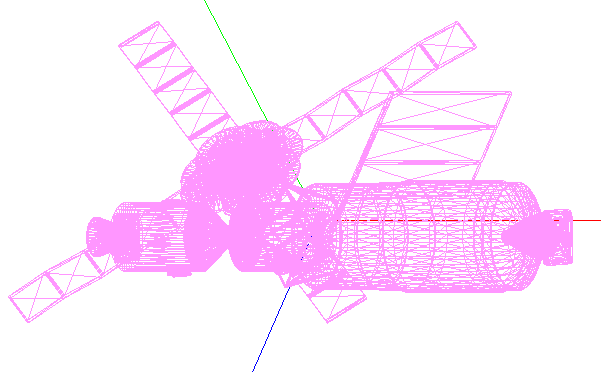
\includegraphics[scale=0.75]{screens/screenshot1.png}
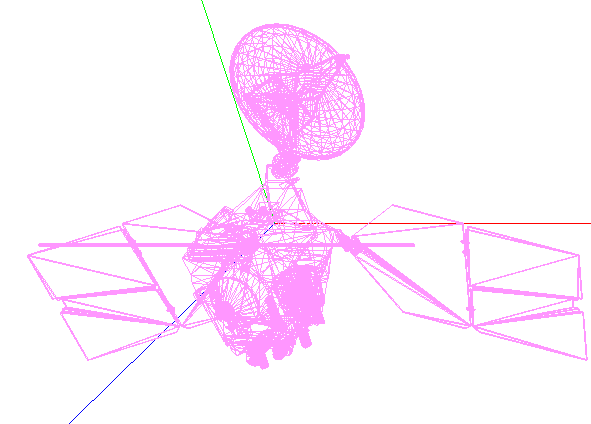
\includegraphics[scale=0.75]{screens/screenshot2.png}
\caption{Моделі космічних апаратів}
\label{}
\end{figure}

\newpage
\subsubsection{Зображення частинок, що моделюються}

\begin{figure}[!htp]
\centering
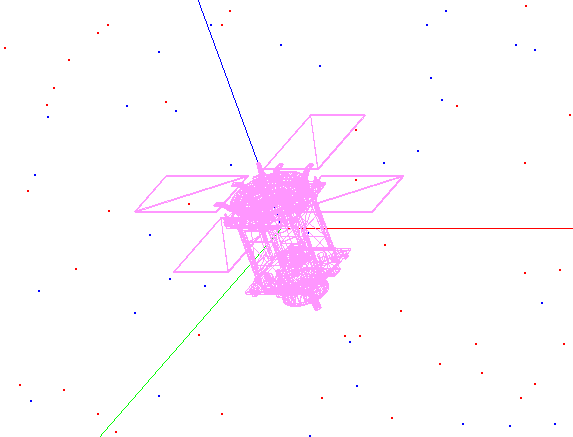
\includegraphics[scale=0.7]{screens/screenshot3.png}
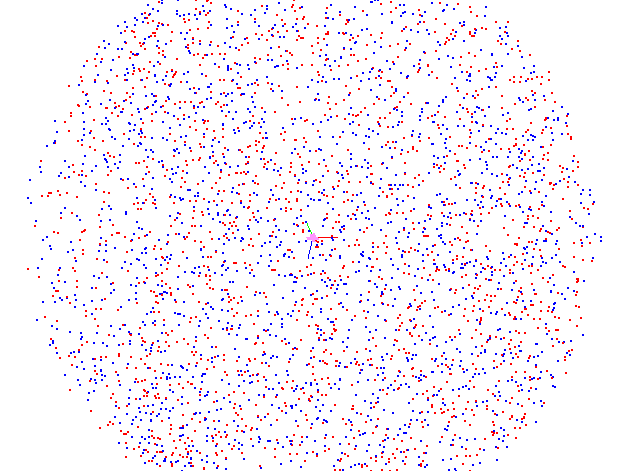
\includegraphics[scale=0.7]{screens/screenshot4.png}
\caption{Моделі космічних апаратів та елементарних частинок}
\label{fig:f2}
\end{figure}
\newpage

На рисунку \ref{fig:f2} зверху показано космічний апарат у наближенні. В нижній частині камеру віддалено достатньо для того, щоб побачити, що все моделювання відбувається в межах сфери.

Також слід зазначити, що сині точки позначають електрони, а червоні -- іони.

\subsubsection{Результати спостережень}
Зміна заряду (за час 0.00025 секунди)
\begin{figure}[!htp]
\centering
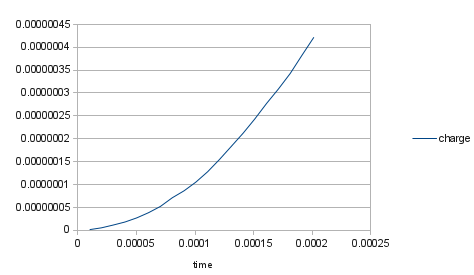
\includegraphics[scale=1.00]{screens/screenshot5.png}
\caption{Зміна заряду}
\end{figure}
\newpage

Зміна потенціалу (за час 0.00025 секунди)
\begin{figure}[!htp]
\centering
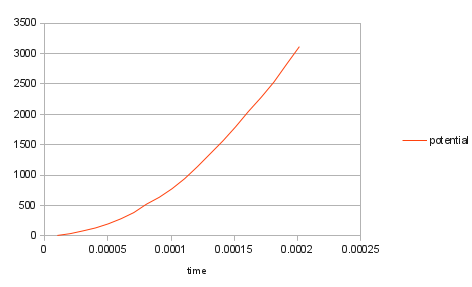
\includegraphics[scale=1.00]{screens/screenshot6.png}
\caption{Зміна потенціалу}
\end{figure}

Сумарна кількість зіткнень частинок (в цифрах реальної системи) з космічним апаратом (за час 0.00025 секунди)
\begin{figure}[!htp]
\centering
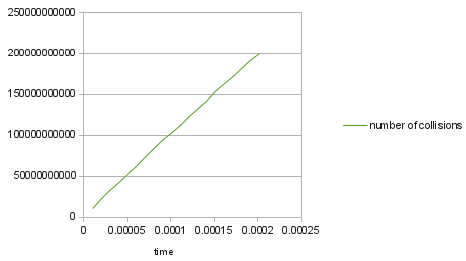
\includegraphics[scale=1.00]{screens/screenshot7.png}
\caption{Сумарна кількість зіткнень}
\end{figure}
\newpage

\newpage

\addcontentsline{toc}{section}{Висновок}
\section*{Висновок}
Було розроблено програмне забезпечення для моделювання руху літального апарату та зіткнення з ним елементарних частинок, що складають космічну плазму.

Отримана програма має зрозумілий інтерфейс командного рядка та формат вихідних даних. Завдяки використанню бібліотеки ASSIMP і власних функцій зчитування здатна працювати з вхідними файлами різноманітних форматів.

В програмі використано також наявні експериментальні дані, що були взяті з відповідної літератури.

За допомогою розробленого програмного забезпечення було проведено моделювання за статистичним методом Монте-Карло, було прослідковано зміну потенціалу космічного апарату і струмів на його поверхні з плином часу, а також кількість зіткнень елементарних частинок з космічним апаратом.

Також розроблена програма здатна візуалізувати процес моделювання, використовуючи графічну бібліотеку OpenGL та бібліотеку роботи з мультимедіа SDL.

Окрім того, розроблені в рамках програми модулі можуть використовуватись окремо від неї, оскільки кожен з них містить завершений функціонал деякого напрямку -- це
\begin{itemize}
  \item модуль з описом структур даних, що представляють геометричні примітиви і фізичні об’єкти
  \item модуль алгоритмів, що дозволяють змоделювати взаємодію цих об’єктів
  \item модуль з функціями для зручної генерації випадкових величин із заданим розподілом і параметрами
  \item невеликий, але зручний модуль обробки масивів даних
  \item модуль зчитування моделей апаратів і збереження їх в описану в програмі структуру
  \item модуль зображення частинок і полігональних об’єктів засобами OpenGL
\end{itemize}

З використанням розробленого програмного забезпечення було змодельовано і досліджено процес електризації космічних апаратів. На основі отриманих даних було побудовано графіки, що відображають залежність різних параметрів системи від часу.

На даному етапі було розглянуто дещо спрощену модель -- струми частинок плазми на поверхні незарядженого тіла, але розроблене програмне забезпечення може слугувати базою для подальших досліджень -- моделюванню руху частинок поблизу тіла, поверхня якого вже має деякий заряд.


\newpage

\addcontentsline{toc}{section}{Література}
\begin{thebibliography}{9}

\bibitem{vakulin}
  Ю.И. Вакулин, О.С. Графодатский, В.И. Гусельников, В.И. Дегтярев, Г.А. Жеребцов, Ш.Н. Исляев, А.А. Кочеев, О.И. Платонов, Г.В. Попов, Л.Л. Фрумин
  \emph{Основные геофизические закономерности электризации геостационарных спутников связи «Горизонт»}

\bibitem{report1}
  А. М. Капулкин, В. Г. Труш, Д. В. Красношапка:
  \emph{Исследование плазменных нейтрализаторов для снятия электростатических зарядов с поверхности высокоорбитальных космических аппаратов}.
  ДНУ, 1994.

\bibitem{sharp}
  Sharp R.D., Shelley E.G., Johonson K.G., Paschmann G.
  \emph{Preliminary Results of a Low Energy Particle Survey at Synchronous Altitude}
  JGR, 1970, Volume 75, P. 6092

\bibitem{deforest}
  DeForest S.E.
  \emph{Spacecraft Charging at Synchronous Altitudes}
  JGR, 1972, Volume 77, P. 651-659

\bibitem{novikov}
  Новиков Л.С.
  \emph{Взаимодействие космических аппаратов с окружающей плазмой}
  Учебное пособие. -- М.: Университетская книга, 2006. -- 120 с.
  
\bibitem{Metropolis}
  Metropolis N., Ulam S.
  \emph{The Monte-Carlo method}
  J. Amer. Stat. Assos. 44,  № 247, 1949

\bibitem{belocerkovskyi}
  О.М. Белоцерковский, Ю.И. Хлопков:
  \emph{Методы Монте-Карло в прикладной математике и вычислительной аэродинамике}.

\bibitem{assimp}
  \url{http://assimp.sourceforge.net/lib_html/index.html}
  \emph{ASSIMP - Open Asset Import Library}
  
\bibitem{nasa}
  \url{http://www.nasa.gov/multimedia/3d_resources/models.html}
  \emph{National Aeronautics and Space Administration}
  
\bibitem{sobol}
  И. М. Соболь:
  \emph{Метод Монте-Карло}.
  «Наука», Москва, 1968.

\end{thebibliography}

\newpage
\addcontentsline{toc}{section}{Додаток}
\section*{Додаток}

\setstretch{0.8}

\lstset{
	basicstyle=\scriptsize,
	tabsize=2,
	breaklines=true,
	title=\lstname,
	showspaces=false,
	showstringspaces=false,
	showtabs=false
} 

\lstinputlisting[language=C++]{dr_program/constants.h}
\lstinputlisting[language=C++]{dr_program/constants.cpp}
\lstinputlisting[language=C++]{dr_program/data_utils.h}
\lstinputlisting[language=C++]{dr_program/file_utils.h}
\lstinputlisting[language=C++]{dr_program/file_utils.cpp}
\lstinputlisting[language=C++]{dr_program/geometry_utils.h}
\lstinputlisting[language=C++]{dr_program/geometry_utils.cpp}
\lstinputlisting[language=C++]{dr_program/graphics_utils.h}
\lstinputlisting[language=C++]{dr_program/graphics_utils.cpp}
\lstinputlisting[language=C++]{dr_program/time_utils.h}
\lstinputlisting[language=C++]{dr_program/time_utils.cpp}
\lstinputlisting[language=C++]{dr_program/types.h}
\lstinputlisting[language=C++]{dr_program/types.cpp}
\lstinputlisting[language=C++]{dr_program/main.cpp}
\end{document}
